\documentclass[12pt]{article}
\usepackage{amsmath}
\usepackage{amssymb}
\usepackage{graphicx}
\usepackage{tabulary}
\usepackage{float}
\usepackage{hyperref}
\usepackage{tikz}
\usetikzlibrary{arrows, decorations.markings}

\tikzstyle{vecArrow} = [thick, decoration={markings,mark=at position
   1 with {\arrow[semithick]{open triangle 60}}},
   double distance=1.4pt, shorten >= 5.5pt,
   preaction = {decorate},
   postaction = {draw,line width=1.4pt, white,shorten >= 4.5pt}]
\tikzstyle{innerWhite} = [semithick, white,line width=1.4pt, shorten >= 4.5pt]

\begin{document}

\title{Final Project}%replace X with the appropriate number
\author{William Harrington, Sheetal Konnur\\ %replace with your name
ECE478} %if necessary, replace with your course title
\date{}
 
\maketitle
\small
\begin{description}
	\item[Introduction] \hfill \\
		This report contains a detailed explanation of the Final project for the Marie Curie group. \\ \\
		\textbf{Goals}
		\begin{enumerate}
			\item Use an arduino to drive the servo controller
			\item Use a raspberry pi 2 to do image processing with a kinect
			\item Interface raspberry pi 2 and arduino
			\item Implement some sort of behavior in the robot based on
			\item Add mechanical support for shoulders
		\end{enumerate}
		\centering
		\tikzstyle{int}=[draw, fill=blue!20, minimum size=2em]
		\tikzstyle{init} = [pin edge={to-,thin,black}]
		\textbf{High level system model} \\
		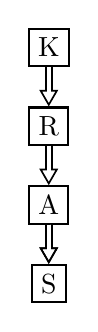
\begin{tikzpicture}[thick]
  			\node[draw,rectangle] (a) {K};
  			
	  		\node[draw,rectangle,below of=a] (b) {R};
  			\node[draw,rectangle,below of=b] (c) {A};
  			\node[draw,rectangle,below of=c] (d) {S};
			
  			% 1st pass: draw arrows
  			\draw[vecArrow] (a) to (b);
  			\draw[vecArrow] (b) to (c);
			\draw[vecArrow] (c) to (d);

  			% 2nd pass: copy all from 1st pass, and replace vecArrow with innerWhite
  			\draw[innerWhite] (a) to (b);
 		 	\draw[innerWhite] (b) to (c);
			\draw[vecArrow] (c) to (d);

  		% Note: If you have no branches, the 2nd pass is not needed
		\end{tikzpicture}
		\begin{itemize}
			\item K = kinect
			\item R = raspberry pi 2
			\item A = Arduino
			\item S = Servo controller
		\end{itemize}
		\newpage
		\textbf{Model of algorithm} \\
		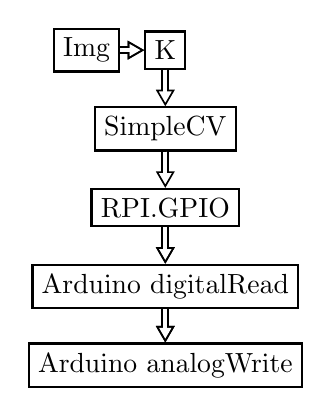
\begin{tikzpicture}[thick]
  			\node[draw,rectangle] (a) {K};
  			
	  		\node[draw,rectangle,below of=a] (b) {SimpleCV};
  			\node[draw,rectangle,below of=b] (c) {RPI.GPIO};
  			\node[draw,rectangle,below of=c] (d) {Arduino digitalRead};
			\node[draw,rectangle,left of=a] (e) {Img};
			\node[draw,rectangle,below of=d] (f) {Arduino analogWrite};
			
  			% 1st pass: draw arrows
  			\draw[vecArrow] (a) to (b);
  			\draw[vecArrow] (b) to (c);
			\draw[vecArrow] (c) to (d);
			\draw[vecArrow] (e) to (a);
			\draw[vecArrow] (d) to (f);

  			% 2nd pass: copy all from 1st pass, and replace vecArrow with innerWhite
  			\draw[innerWhite] (a) to (b);
 		 	\draw[innerWhite] (b) to (c);
			\draw[vecArrow] (c) to (d);
			\draw[vecArrow] (e) to (a);
			\draw[vecArrow] (d) to (f);

  		% Note: If you have no branches, the 2nd pass is not needed
		\end{tikzpicture}
		\begin{itemize}
			\item Img = Image
			\item K = kinect
			\item SimpleCV = Python wrappers for OpenCV
			\item RPI.GPIO = Python wrappers for controlling Raspberry Pi GPIO pins
			\item Arduino digitalRead = Arduino function to read if pin is high or low
			\item Arduino analogWrite = Arduino function for Pulse Width Modulation on capable pin
		\end{itemize}
\end{description}

\end{document}